\documentclass[aspectratio=169,usenames,dvipsnames]{beamer}
\usepackage{preamble}
\title{Coding for Humanities, week 5}

\begin{document}

\begin{frame}
 \titlepage
\end{frame}

\begin{frame}{Last week}
    Files \& directories

    Libraries
\end{frame}

\begin{frame}{Plan for today}
 \tableofcontents
\end{frame}

\section{The Midterm}
\begin{frame}
    \begin{reference}
        \hfill Source: \url{https://oktop.tumblr.com/post/15352780846}
    \end{reference}
    \begin{columns}[b]
        \column{0.5\linewidth}
            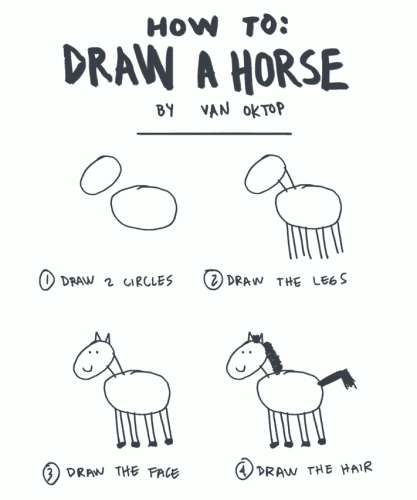
\includegraphics[height=0.9\textheight]{fig/horse1}
        \pause
        \column{0.5\linewidth}
            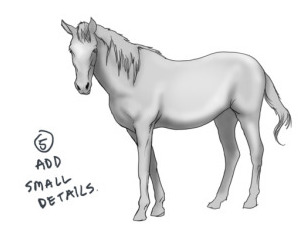
\includegraphics[width=0.9\linewidth]{fig/horse2}
    \end{columns}
\end{frame}


\section{Improving code}
\subsection{Making it work}
\frame{\tableofcontents[currentsection]}
\begin{frame}
    \begin{definition}
        \structure{Debugging}: identifying and remove errors in programs
    \end{definition}

    \pause

    ``If debugging is the art of removing bugs from programs,
    programming must be the art of inserting them''

\end{frame}

\begin{frame}{Common errors}
    \begin{description}
        \item[SyntaxError] ...
        \item[NameError] ...
        \item[TypeError] ...
        \item[ValueError] ...
        \item[IndexError] ...
        \item[KeyError] ...
        \item[AttributeError] ...
        \item[...] ...
    \end{description}
\end{frame}

\subsection{Making it better}
\frame{\tableofcontents[currentsection]}

\begin{frame}{Refactoring}
	Insight: can achieve the same end in many different ways

	\pause
	\begin{definition}
		\structure{Refactoring}: improving code (e.g., readability) \\
			while keeping the same functionality (i.e., behavior).
	\end{definition}

	\begin{itemize}
		\item Clear variable names
		\item Separate steps
        \item Use idioms
	\end{itemize}
\end{frame}

\subsection{Making it faster}
\frame{\tableofcontents[currentsection]}
\begin{frame}{Profiling}
	\begin{definition}
		\structure{Profiling}: identify bottlenecks by measuring
	\end{definition}

	\begin{itemize}
		\item Avoid doing unnecessary things
		\item Avoid slow methods
	\end{itemize}
\end{frame}

\section{Counting particular words}
\subsection{Sentiment analysis}
\frame{\tableofcontents[currentsection]}

\begin{frame}{}
	\begin{definition}
        \structure{Sentiment (polarity) analysis}: 
            is a piece of language positive or negative?
	\end{definition}

	\begin{itemize}
		\item 
		\item 
	\end{itemize}

    % Show how to use sentiment word lists
    % Show example applications in literature
\end{frame}

\subsection{Keyword analysis}
\begin{frame}{}
	\begin{definition}
		\structure{Keyword}: a word that is statistically characteristic of a text.
	\end{definition}

	\begin{itemize}
		\item Identify important topics
		\item 
	\end{itemize}

    % Show how to find keywords with NLTK
    % Example applications in ...
\end{frame}

\end{document}
